\chapter{Preparación del entorno de la máquina virtual}

Partiremos de la máquina virtual proporcionada por el profesor, la cual tiene instalado el sistema operativo Ubuntu 22.04.3 LTS.

\section{Preparación de Cassandra}

Primero instalaremos Cassandra, para ello primero actualizaremos el sistema operativo. El comando \texttt{sudo apt update} actualiza la lista de paquetes disponibles y sus versiones, mientras que el comando \texttt{sudo apt upgrade} instala las actualizaciones disponibles.

\begin{lstlisting}[language=bash]
sudo apt update && sudo apt upgrade
\end{lstlisting}

\begin{figure}[H]
    \centering
    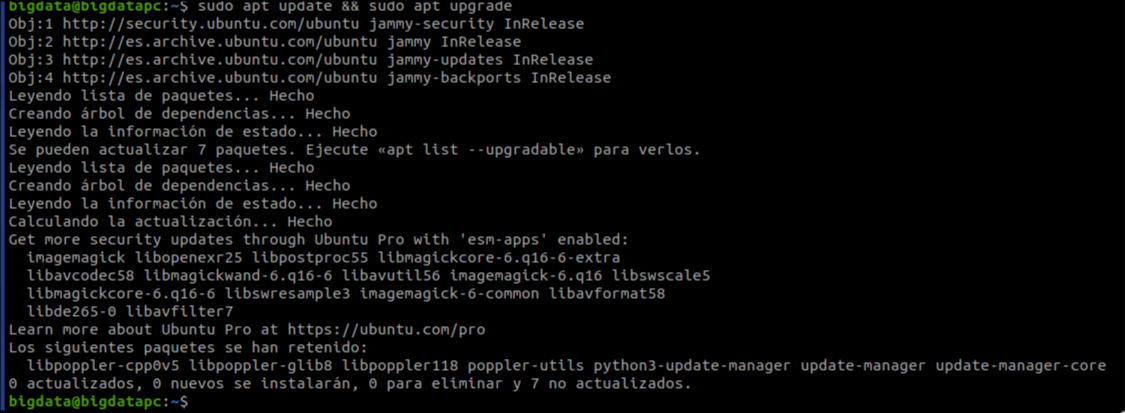
\includegraphics[width=0.8\textwidth]{figures/1.png}
    \caption{Actualización del sistema operativo}
\end{figure}

Ahora instalaremos Python 2, ya que Cassandra requiere esta versión de Python. Para ello, ejecutamos el siguiente comando:

\begin{lstlisting}[language=bash]
sudo apt install python2
\end{lstlisting}

\begin{figure}[H]
    \centering
    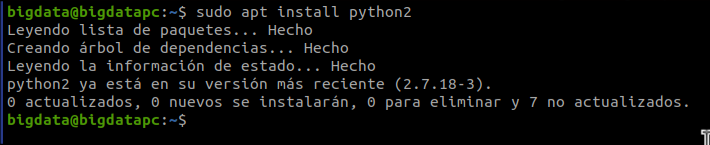
\includegraphics[width=0.8\textwidth]{figures/2.png}
    \caption{Instalación de Python 2}
\end{figure}

Después, descargaremos el archivo .tar.gz de Cassandra desde la página oficial de Apache. Para ello, ejecutamos el siguiente comando:

\begin{lstlisting}[language=bash]
    wget https://dlcdn.apache.org/cassandra/3.11.16/apache-cassandra-3.11.16-bin.tar.gz
\end{lstlisting}

\begin{figure}[H]
    \centering
    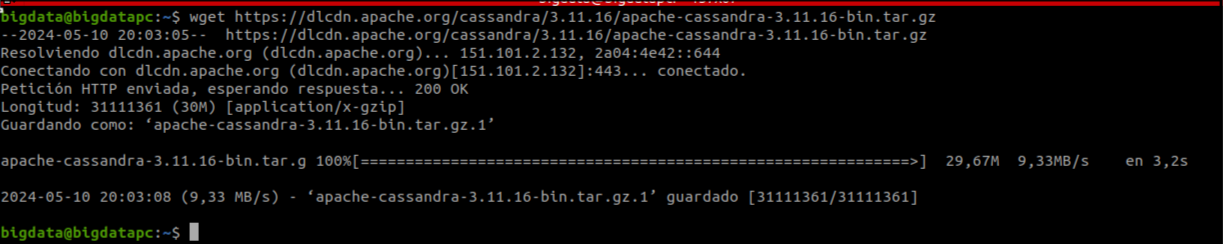
\includegraphics[width=0.8\textwidth]{figures/3.png}
    \caption{Descarga de Cassandra}
\end{figure}

Descomprimimos el archivo .tar.gz con el siguiente comando:

\begin{lstlisting}[language=bash]
    tar -xvzf apache-cassandra-3.11.16-bin.tar.gz
\end{lstlisting}

\begin{figure}[H]
    \centering
    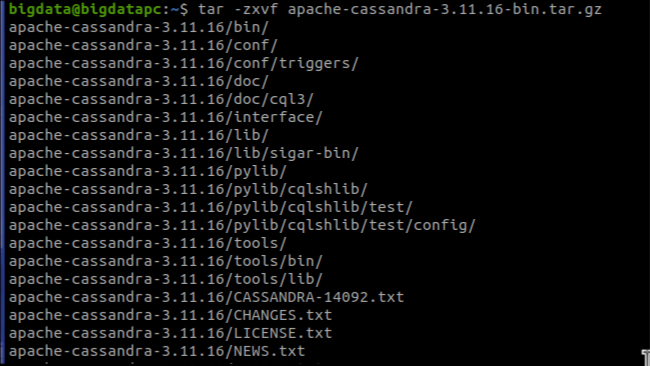
\includegraphics[width=0.8\textwidth]{figures/4.png}
    \caption{Descompresión de Cassandra}
\end{figure}

Por último, eliminamos el archivo .tar.gz con el siguiente comando:

\begin{lstlisting}[language=bash]
    rm apache-cassandra-3.11.16-bin.tar.gz
\end{lstlisting}

\begin{figure}[H]
    \centering
    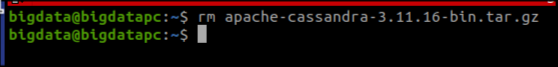
\includegraphics[width=0.8\textwidth]{figures/5.png}
    \caption{Eliminación del archivo .tar.gz}
\end{figure}

\chapter{Desplegar HDFS}

HDFS ya está instalado por defecto en la máquina virtual en la carpeta \texttt{~/hadoop-3.3.6}. Para desplegar HDFS ejecutamos el siguiente comando:

\begin{lstlisting}[language=bash]
    ~/hadoop-3.3.6/sbin/start-dfs.sh
\end{lstlisting}

\begin{figure}[H]
    \centering
    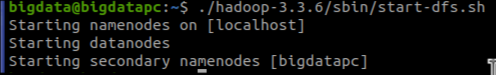
\includegraphics[width=0.8\textwidth]{figures/6.png}
    \caption{Despliegue de HDFS}
\end{figure}

Ahora para comprobar que HDFS se ha desplegado correctamente, ejecutamos el siguiente comando:

\begin{lstlisting}[language=bash]
    jps
\end{lstlisting}

\begin{figure}[H]
    \centering
    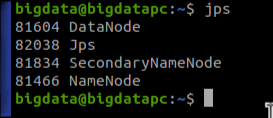
\includegraphics[width=0.8\textwidth]{figures/7.png}
    \caption{Comprobación de HDFS}
\end{figure}

Ahora ya podemos ejecutar comandos de HDFS, como por ejemplo el siguiente comando que muestra los archivos en el sistema de archivos HDFS:

\begin{lstlisting}[language=bash]
    ~/hadoop-3.3.6/bin/hdfs dfs -ls /
\end{lstlisting}

\begin{figure}[H]
    \centering
    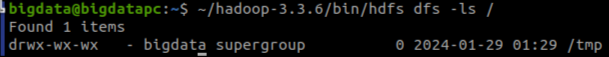
\includegraphics[width=0.8\textwidth]{figures/8.png}
    \caption{Comando de HDFS}
\end{figure}

\chapter{Desplegar PostgreSQL}

Postgres también está instalado por defecto en la máquina virtual, además se arranca por defecto al iniciar la sesión en la máquina virtual. Para comprobar que Postgres se ha desplegado correctamente, ejecutamos el siguiente comando:

\begin{lstlisting}[language=bash]
    sudo systemctl status postgresql
\end{lstlisting}
